\begin{appendices}
\crefalias{chapter}{appendix}
\startcontents[chapters]

\chapter{Peripheral Information}
\startcontents[chapters]
\printcontents[chapters]{}{1}{}
\noindent\\
To provide user's with useful functionality, common system-on-chip peripherals were created. This section describes each peripheral and it's design decisions. The full memory-map is shown in \cref{fig:memmap}.

\section{Special Registers}
From the software perspective, it is important for both the developer and software algorithms to know the target system's architecture to better utilise
the resources available to them.
Software written for one architecture with $N$ cores must also run on an architecture with $M$ cores. To enable such portability, the software must query the system for information such as: number of processor cores and the current core identifier. Without this information, the developer would be required to produce software for each individual architecture (e.g. an Intel i5 with 4 cores or an Intel i7 with 8 cores, or an NVIDIA GTX 970 with 1664 CUDA cores.

The special register peripheral is shown below.

\begin{figure}[H]
\centering
\begin{bytefield}[bitwidth=4ex, rightcurly=., rightcurlyspace=0pt]{16}
\bitheader[endianness=big]{0-15} \\
\begin{rightwordgroup}{0080 R}
\bitbox{8}{\color{lightgray}\rule{\width}{\height}} & \bitbox{8}{CORE\_ID}
\end{rightwordgroup} \\
\begin{rightwordgroup}{0081 R}
\bitbox{8}{\color{lightgray}\rule{\width}{\height}} & \bitbox{8}{NUM\_CORES}
\end{rightwordgroup} \\
\begin{rightwordgroup}{0082 R}
\bitbox{16}{SHARED\_MEMORY cells \tiny(default 4096)}
\end{rightwordgroup} \\
\begin{rightwordgroup}{0083 R}
\bitbox{8}{\color{lightgray}\rule{\width}{\height}} & \bitbox{8}{NUM\_PERIPHERALS}
\end{rightwordgroup} \\
\begin{rightwordgroup}{0084 RW}
\bitbox{16}{SCRATCH\_MEMORY cells \tiny(default 64)}
\end{rightwordgroup} \\
\begin{rightwordgroup}{0085 RW}
\bitbox{16}{User defined}
\end{rightwordgroup} \\
\bitbox[]{16}{$\vdots$ \\[1ex]} \\
\begin{rightwordgroup}{008F RW}
\bitbox{16}{User defined}
\end{rightwordgroup}
\end{bytefield}
\caption{Vmicro16 Special Registers layout (0x0080 - 0x008F).}
\end{figure}

\section{Watchdog Timer}
\label{sect:watchdog}
In any multi-threaded system there exists the possibility for a deadlock -- a state where all threads are in a waiting state -- and algorithm execution is forever blocked. This can occur either by poor software programming or incorrect thread arbitration by the processor. A common method of detecting a deadlock is to make each thread signal that it is not blocked by resetting a countdown timer. If the countdown timer is not reset, it will eventually reach zero and it is assumed that all threads are blocked as none have reset the countdown.

In this system-on-chip design, software can reset the watchdog timer by writing any 16-bit value to the address \verb|0x00B8|.

This peripheral is optional and can be enabled using the configuration parameters described in \nameref{sect:config}.

\begin{figure}[H]
\centering
\begin{bytefield}[bitwidth=4ex, rightcurly=., rightcurlyspace=0pt]{16}
\bitheader[endianness=big]{0-15} \\
\begin{rightwordgroup}{00B8 W}
\bitbox{16}{Reset Watchdog}
\end{rightwordgroup}
\end{bytefield}
\end{figure}

\section{GPIO Interface}
\begin{figure}[H]
\centering
\begin{bytefield}[bitwidth=4ex, rightcurly=., rightcurlyspace=0pt]{16}
\bitheader[endianness=big]{0-15} \\
\begin{rightwordgroup}{0090 RW}
\bitbox{8}{\color{lightgray}\rule{\width}{\height}} &
\bitbox{8}{GPIO0 Output}
\end{rightwordgroup} \\
\begin{rightwordgroup}{0091 RW}
\bitbox{16}{GPIO1 Output}
\end{rightwordgroup} \\
\begin{rightwordgroup}{0092 RW}
\bitbox{8}{\color{lightgray}\rule{\width}{\height}} &
\bitbox{8}{GPIO2 Output}
\end{rightwordgroup}\\
\begin{rightwordgroup}{0093 R}
\bitbox{8}{\color{lightgray}\rule{\width}{\height}} &
\bitbox{8}{GPIO3 Input}
\end{rightwordgroup}
\end{bytefield}
\end{figure}
On the DE1-SoC board, GPIO0 is assigned to the LEDs, and GPIO1 and GPIO2 to the 6 seven-segment displays.


\section{Timer with Interrupt}
\label{sect:timer}
\begin{figure}[H]
\centering
\begin{bytefield}[bitwidth=4ex, rightcurly=., rightcurlyspace=0pt]{16}
\bitheader[endianness=big]{0-15} \\
\begin{rightwordgroup}{0200 RW}
\bitbox{16}{Load Value}
\end{rightwordgroup} \\
\begin{rightwordgroup}{0201 W}
\bitbox{13}{\color{lightgray}\rule{\width}{\height}} &
\bitbox{1}{I} &
\bitbox{1}{R} &
\bitbox{1}{S}
\end{rightwordgroup} \\
\begin{rightwordgroup}{0202 W}
\bitbox{16}{Prescaler}
\end{rightwordgroup}
\end{bytefield}
\end{figure}

\begin{description}
\item [Clock Frequency] Uses top level FPGA clock (normally 50 MHz).
\item [Load Value] Value to count down from each clock.
\item [I] Interrupt enable bit. Default 0.
\item [R] Reset Load Value and Prescaler values to their last written value.
\item [S] Start the timer countdown. 1 = start. 0 = stop.
\item [Prescaler]  Number of clocks per FPGA clock to wait between each decrement.
\end{description}


\section{UART Interface}
\begin{figure}[H]
\centering
\begin{bytefield}[bitwidth=4ex, rightcurly=., rightcurlyspace=0pt]{16}
\bitheader[endianness=big]{0,1,7,8,15} \\
\begin{rightwordgroup}{00A0 W}
\bitbox{8}{\color{lightgray}\rule{\width}{\height}} & \bitbox{8}{Transmit Data}
\end{rightwordgroup} \\
\begin{rightwordgroup}{00A1 R}
\bitbox{8}{\color{lightgray}\rule{\width}{\height}} & \bitbox{8}{Receive Data}
\end{rightwordgroup} \\
\begin{rightwordgroup}{00A2 RW}
\bitbox{14}{\color{lightgray}\rule{\width}{\height}} & \bitbox{1}{E} & \bitbox{1}{I}
\end{rightwordgroup}
\end{bytefield}
\end{figure}

\begin{description}
\item [E] Enable the UART  component.
\item [I] Enable an interrupt upon receiving new data. Default 1.
\end{description}

\begin{quote}
Note: If \verb|DEF_USE_REPROG| is enabled in \verb|vmicro16_soc_config.v| then the Receive Data register will be reserved for programming the instruction memory, resulting in reads and writes to addresses 0x00A1 and 0x00A2 to return 0.
\end{quote}


\chapter{Additional Figures}

\begin{listing}[H]
\centering
\begin{minted}[fontsize=\footnotesize]{verilog}
input      [MASTER_PORTS*BUS_WIDTH-1:0]  S_PADDR,
input      [MASTER_PORTS-1:0]            S_PWRITE,
input      [MASTER_PORTS-1:0]            S_PSELx,
input      [MASTER_PORTS-1:0]            S_PENABLE,
input      [MASTER_PORTS*DATA_WIDTH-1:0] S_PWDATA,
output reg [MASTER_PORTS*DATA_WIDTH-1:0] S_PRDATA,
output reg [MASTER_PORTS-1:0]            S_PREADY,
\end{minted}
\caption{Variable size inputs and outputs to the interconnect.}
\label{lst:widemaster}
\end{listing}

\section{Register Set Multiplex}
\begin{figure}[H]
\centering
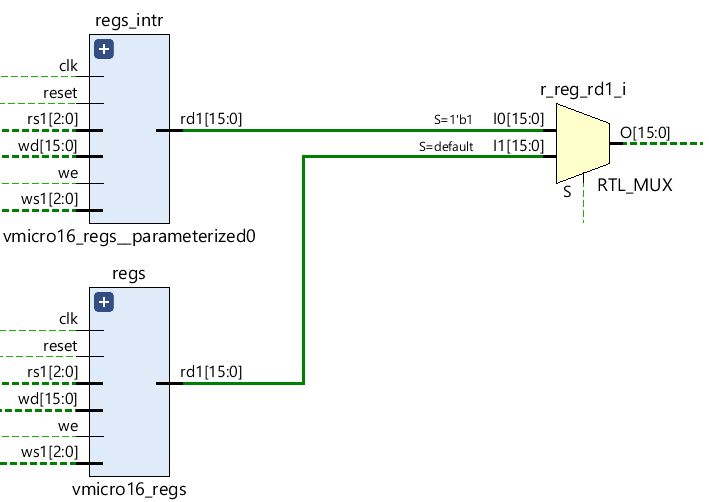
\includegraphics[width=0.7\textwidth]{interrupt_mux}
\caption{Normal mode (bottom) and interrupt mode (top) register sets are multiplexed to switch between contexts.}
\label{fig:regmult}
\end{figure}


\section{Instruction Set Architecture}
\begin{figure}[H]
\centering
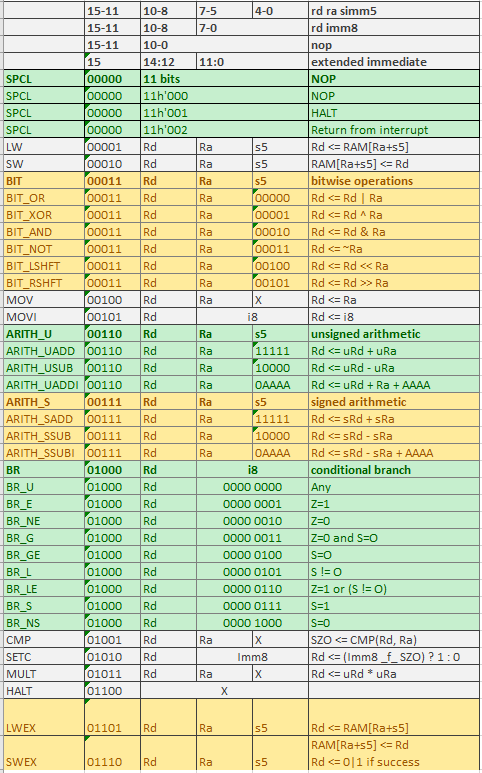
\includegraphics[width=0.7\textwidth]{isa2}
\caption{Vmicro16 instruction set architecture.}
\label{fig:isa}
\end{figure}

\chapter{Configuration Options}
\label{sect:config}
\startcontents[chapters]
\printcontents[chapters]{}{1}{}

\noindent\\
The following configuration options are defined in \verb|vmicro16_soc_config.v|.

\begin{quote}
Defaults with empty/blank values signifies that the preprocessor define is commented out/not defined/disabled by default/computed by other parameters.
\end{quote}

\section{System-on-Chip Configuration Options}
\begin{table}[H]
\centering
\begin{tabularx}{\textwidth}{l|l|p{8cm}}
Macro      & Default & Purpose                         \\ 
\hline
CORES  & 4       & Number of CPU cores in the SoC  \\
SLAVES & 9       & Number of peripherals  \\    
DEF\_USE\_WATCHDOG & //  & Enable watchdog module to recover from deadlocks and infinite loops. Requires DEF\_GLOBAL\_RESET. \\
DEF\_GLOBAL\_RESET           & //      & Enable synchronous reset logic. Will consume more LUT resources. Does not reset BRAM blocks.\\
DEF\_USE\_BUS\_RESET & //      & Detect bus stalls or errors to soft-reset the whole design. Requires DEF\_USE\_WATCHDOG.\\
\end{tabularx}
\caption{SoC Configuration Options}
\end{table}

\section{Core Options}
\begin{table}[H]
\centering
\begin{tabular}{l|l|p{8cm}}
Macro                      & Default & Purpose                                     \\ 
\hline
DATA\_WIDTH                & 16      & Width of CPU registers in bits              \\
DEF\_CORE\_HAS\_INSTR\_MEM & //      & Enable a per core instruction memory cache  \\
DEF\_MEM\_INSTR\_DEPTH     & 64      & Instruction memory cache per core           \\
DEF\_MEM\_SCRATCH\_DEPTH   & 64      & RW RAM per core                             \\
DEF\_ALU\_HW\_MULT        & 1       & Enable/disable HW multiply (1 clock)         \\
FIX\_T3                    & //      & Enable a T3 state for the APB transaction   \\
DEF\_USE\_REPROG           & //      & Programme instruction memory via UART0. Requires DEF\_GLOBAL\_RESET. Enabling this will reserve the UART0 RX port for exclusive use for programming the instruction memory. Software reads of UART0 RX will return 0.\\
\end{tabular}
\caption{Core Options}
\end{table}

\section{Peripheral Options}
\begin{table}[H]
\centering
\begin{tabular}{l|l|l}
Macro              & Default  & Purpose                                              \\ 
\hline
APB\_WIDTH         &          & AMBA APB PADDR signal width                          \\
APB\_PSELX\_GPIO0  & 0        & GPIO0 index                                          \\
APB\_PSELX\_UART0  & 1        & UART0 index                                          \\
APB\_PSELX\_REGS0  & 2        & REGS0 index                                          \\
APB\_PSELX\_BRAM0  & 3        & BRAM0 index                                          \\
APB\_PSELX\_GPIO1  & 4        & GPIO1 index                                          \\
APB\_PSELX\_GPIO2  & 5        & GPIO2 index                                          \\
APB\_PSELX\_TIMR0  & 6        & TIMR0 index                                          \\
APB\_BRAM0\_CELLS  & 4096     & Shared memory words                                  \\
DEF\_MMU\_TIM0\_S  & 16'h0000 & Per core scratch memory start/end address            \\
DEF\_MMU\_TIM0\_E  & 16'h007F & "                                                    \\
DEF\_MMU\_SREG\_S  & 16'h0080 & Per core special registers start/end address         \\
DEF\_MMU\_SREG\_E  & 16'h008F & "                                                    \\
DEF\_MMU\_GPIO0\_S & 16'h0090 & Shared GPIOn start/end address                       \\
DEF\_MMU\_GPIO0\_E & 16'h0090 & "                                                    \\
DEF\_MMU\_GPIO1\_S & 16'h0091 & "                                                    \\
DEF\_MMU\_GPIO1\_E & 16'h0091 & "                                                    \\
DEF\_MMU\_GPIO2\_S & 16'h0092 & "                                                    \\
DEF\_MMU\_GPIO2\_E & 16'h0092 & "                                                    \\
DEF\_MMU\_UART0\_S & 16'h00A0 & Shared UART start/end address                        \\
DEF\_MMU\_UART0\_E & 16'h00A1 & "                                                    \\
DEF\_MMU\_REGS0\_S & 16'h00B0 & Shared registers start/end address                   \\
DEF\_MMU\_REGS0\_E & 16'h00B7 & "                                                    \\
DEF\_MMU\_BRAM0\_S & 16'h1000 & Shared memory with global monitor start/end address  \\
DEF\_MMU\_BRAM0\_E & 16'h1FFF & "                                                    \\
DEF\_MMU\_TIMR0\_S & 16'h0200 & Shared timer peripheral start/end address            \\
DEF\_MMU\_TIMR0\_E & 16'h0202 & "                                                   
\end{tabular}
\caption{Peripheral Options}
\end{table}

\chapter{Viva Demonstration Examples}
\label{sec:vivademos}
\startcontents[chapters]
\printcontents[chapters]{}{1}{}

\section{2-core Timer Interrupt and ISR}
\label{sec:2coretimer}
This example demo, shown during the viva, blinks an LED every 0.5 seconds via a timer interrupt. Core 0 sets up the interrupt vector (by writing the isr0 function address to the interrupt vector) and enables all interrupt sources. Core 1 sets up the timer interval peripheral to produce an interrupt every 0.5 seconds. Core 1 also performs the interrupt handler (isr0): toggle an LED, write the state to UART0, and resets the watchdog.
\inputminted[
    linenos,
    fontsize=\scriptsize,
    baselinestretch=0.8,
]{arm}{../../sw/demos/asm/interrupts_2.s}

\clearpage
\section{1-160 Core Parallel Summation}
\label{sec:64coresum}
This example demo performs a parallel summation of numbers 1 to 320. The algorithm \textit{assigns} each core a subset of the summation space. It does this using the core's ID and the number of cores in the system. The following formulas determine where the subset begins and ends for each core. Core 0 broadcasts the number to sum to then each core calculates its subset start and end positions. Each core then performs a summation over it's subset then adds the result to a global shared value. After pushes it's results, the global shared value will contain the final summation result.
\begin{eqnarray}
N_{samples} = 320\\
N_{threads} = 64\\
subset = N_{samples} / N_{threads}\\
start  = ID * subset\\
end  = start + subset
\end{eqnarray}

\inputminted[
    linenos,
    fontsize=\scriptsize,
    baselinestretch=0.8,
]{arm}{../../sw/demos/asm/sum64.s}

\chapter{Code Listing}
\startcontents[chapters]
\printcontents[chapters]{}{1}{}

\section{SoC Code Listing}
\subsection{vmicro16\_soc\_config.v}
Configuration file for configuring the vmicro16\_soc.v and vmicro16.v features.

\inputminted[
    linenos,
    fontsize=\scriptsize,
    baselinestretch=0.8,
]{verilog}{../../vmicro16/vmicro16_soc_config.v}

\subsection{top\_ms.v}
Top level module that connects the SoC design to hardware pins on the FPGA.
\inputminted[
    linenos,
    fontsize=\scriptsize,
    baselinestretch=0.8,
]{verilog}{../../vmicro16/top_ms.v}

\subsection{vmicro16\_soc.v}
\inputminted[
    linenos,
    fontsize=\scriptsize,
    baselinestretch=0.8,
]{verilog}{../../vmicro16/vmicro16_soc.v}


\subsection{vmicro16.v}
Vmicro16 CPU core module.

\inputminted[
    linenos,
    fontsize=\scriptsize,
    baselinestretch=0.8,
]{verilog}{../../vmicro16/vmicro16.v}

\section{Peripheral Code Listing}
Various memory-mapped APB peripherals, such as GPIO, UART, timers, and memory.

\inputminted[
    linenos,
    fontsize=\scriptsize,
    baselinestretch=0.8,
]{verilog}{../../vmicro16/vmicro16_periph.v}


\section{Assembly Compiler Listing}
The following python3 program is a text assembly to hex compiler for the Vmicro16's instruction. Users can include the compiled hex-stream in their SoC design by using \verb|$readmemh| on the file into the instruction memories (\verb|mem_instr| or \verb|instr_rom_apb| (shared)).

All assembly programs shown in this report can be compiled by this compiler.
\\\\
Usage: \verb|python3 asm.py <filename.s>|\\
Outputs: \verb|asm.s.hex| file in the PWD.

\inputminted[
    linenos,
    fontsize=\scriptsize,
    baselinestretch=0.8,
]{python}{../../sw/asm.py}

\newpage
\section{Text Compiler Listing}
A text-based programming language compiler was also used to write high-level software code for the Vmicro16 processor. The PRCO304 \cite{prco304} compiler was extended to support the Vmicro16 instruction set architecture and some extra language features (arrays, inline assembly, pointer writing, etc.). However, the compiler ended up not being not used in favour of the assembly compiler which could be easily used to write multi-threaded code.
\\\\
The code changes to extend the compiler are available as a \verb|.patch| for users to patch the compiler themselves. The patch is available from: \url{https://github.com/bendl/vmicro16/tree/master/sw/patch}.
\\\\
Code files are found in \verb|sw/demos/prco/*.prco|.
\end{appendices}